\documentclass[a4paper]{article}
\usepackage{graphicx}
\usepackage{amsmath,amssymb,amstext}


\begin{document}

\subsubsection{CompareChildrenMatchedOrSimilar}

  \begin{description}
  
  \item[testcase\_01:] Kein Knoten ist gematched. Alle Similarities betragen 0.
    
   \begin{equation*}
   Similarity = \frac{0+0+0}{3}=0
   \end{equation*}

  
    
	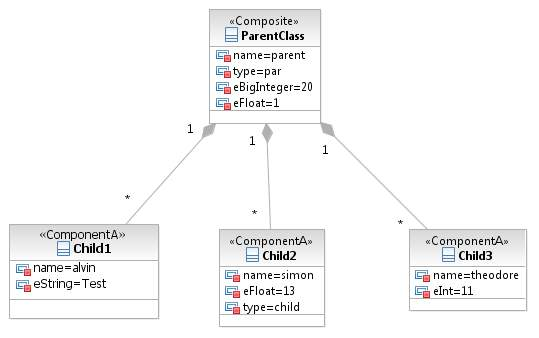
\includegraphics[scale=0.5]{CompareChildrenMatchedOrSimilarTestScreens/Testcase01model1.jpeg}
	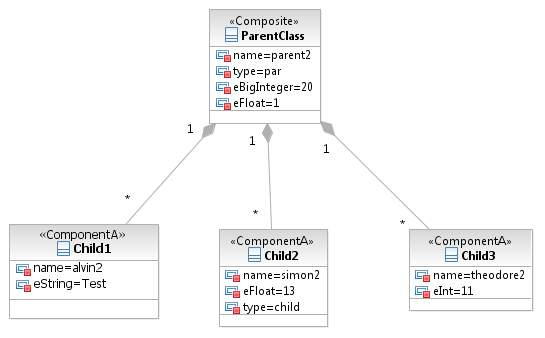
\includegraphics[scale=0.5]{CompareChildrenMatchedOrSimilarTestScreens/Testcase01model2.jpeg}

  \item[testcase\_02:] Alle Knoten sind gematched.    
    
   \begin{equation*}
   Similarity = \frac{1+1+1}{3}=1
   \end{equation*}
    
	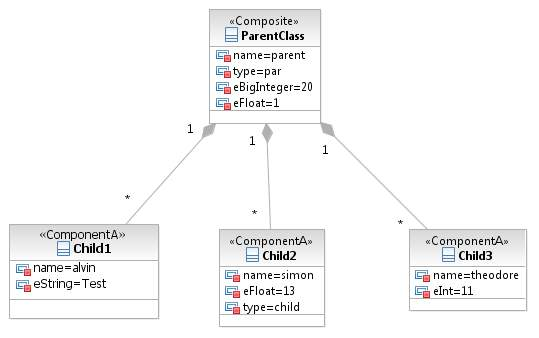
\includegraphics[scale=0.5]{CompareChildrenMatchedOrSimilarTestScreens/Testcase01model1.jpeg}
	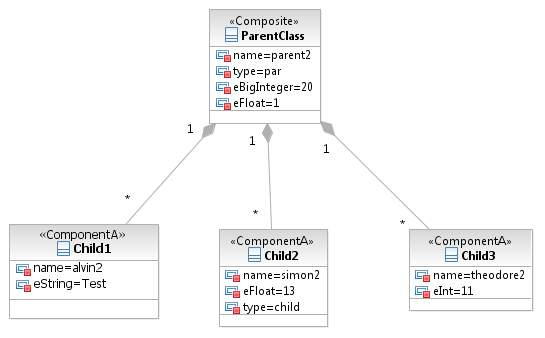
\includegraphics[scale=0.5]{CompareChildrenMatchedOrSimilarTestScreens/Testcase01model2.jpeg}

  \item[testcase\_03:] 2 Kinder gematched. 1 Kind zu 0.5 �hnlich.
    
   \begin{equation*}
   Similarity = \frac{1+1+0.5}{3}=\frac{5}{6}
   \end{equation*}
    
	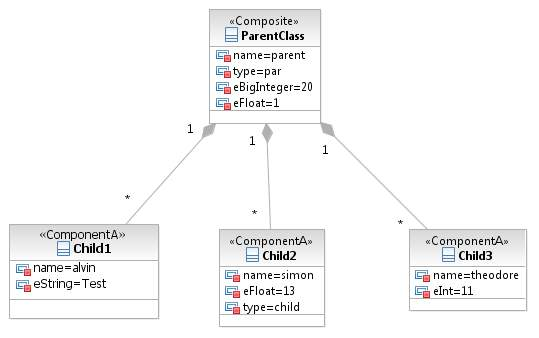
\includegraphics[scale=0.5]{CompareChildrenMatchedOrSimilarTestScreens/Testcase03model1.jpeg}
	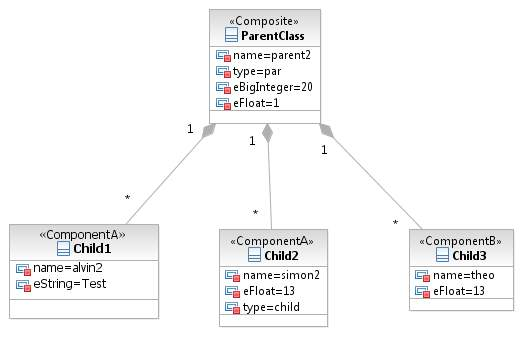
\includegraphics[scale=0.5]{CompareChildrenMatchedOrSimilarTestScreens/Testcase03model2.jpeg}

  \item[testcase\_04:]  1 Kind ist gematched. 1 Kind ist nicht gematched. 1 Kind zu 0.5 �hnlich.
    
   \begin{equation*}
   Similarity = \frac{1+0+0.5}{3}=\frac{1}{2}
   \end{equation*}
    
	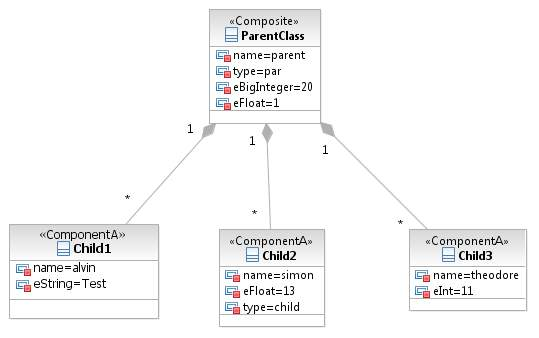
\includegraphics[scale=0.5]{CompareChildrenMatchedOrSimilarTestScreens/Testcase03model1.jpeg}
	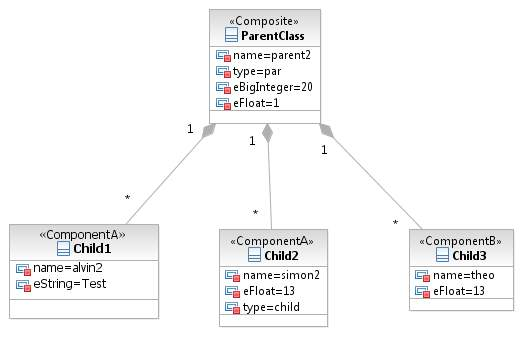
\includegraphics[scale=0.5]{CompareChildrenMatchedOrSimilarTestScreens/Testcase03model2.jpeg}

  \item[testcase\_05:]  1 Kind ist gematched. 1 Kind ist nicht gematched. 1 Kind fehlt (vergleich NULL).
    
   \begin{equation*}
   Similarity = \frac{1+0+0}{3}=\frac{1}{3}
   \end{equation*}
    
	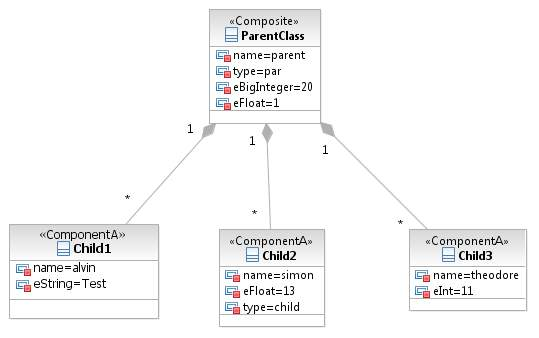
\includegraphics[scale=0.5]{CompareChildrenMatchedOrSimilarTestScreens/Testcase05model1.jpeg}
	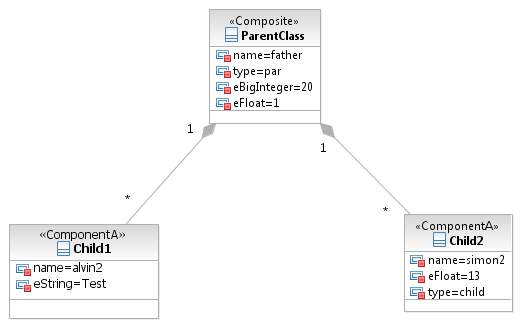
\includegraphics[scale=0.5]{CompareChildrenMatchedOrSimilarTestScreens/Testcase05model2.jpeg}

  \item[testcase\_06:]  2 Kinder sind gematched. 1 Kind fehlt (vergleich NULL).
    
   \begin{equation*}
   Similarity = \frac{1+1+0}{3}=\frac{2}{3}
   \end{equation*}
    
	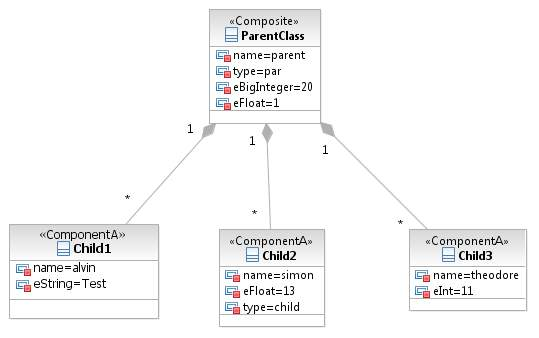
\includegraphics[scale=0.5]{CompareChildrenMatchedOrSimilarTestScreens/Testcase05model1.jpeg}
	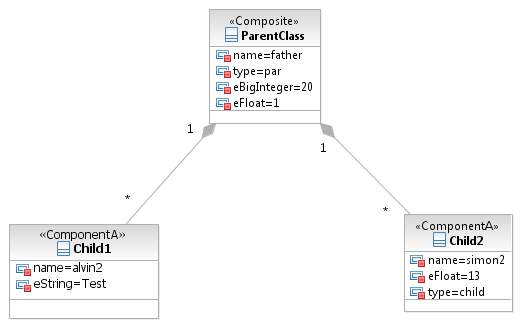
\includegraphics[scale=0.5]{CompareChildrenMatchedOrSimilarTestScreens/Testcase05model2.jpeg}

  \item[testcase\_07:] 3 Kinder sind gematched
    
   \begin{equation*}
   Similarity = \frac{1+1+1}{3}=1
   \end{equation*}
    
	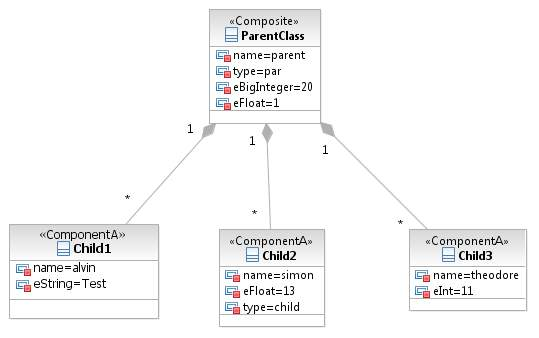
\includegraphics[scale=0.5]{CompareChildrenMatchedOrSimilarTestScreens/Testcase07model1.jpeg}
	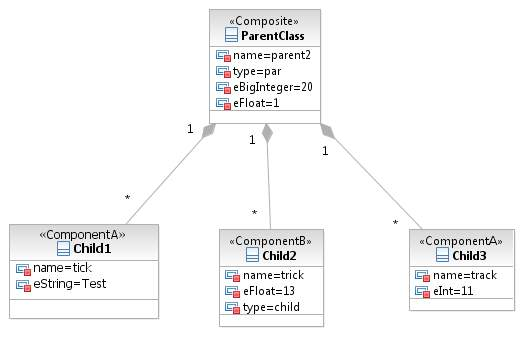
\includegraphics[scale=0.5]{CompareChildrenMatchedOrSimilarTestScreens/Testcase07model2.jpeg}

  \item[testcase\_08] 2 Kinder gematched. 1 Kind zu 100\% �hnlich.
    
   \begin{equation*}
   Similarity = \frac{1+1+1}{3}=1
   \end{equation*}
    
	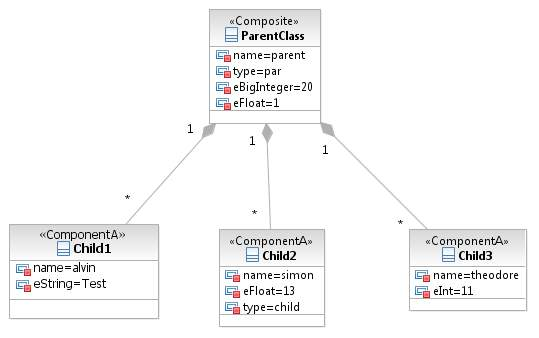
\includegraphics[scale=0.5]{CompareChildrenMatchedOrSimilarTestScreens/Testcase07model1.jpeg}
	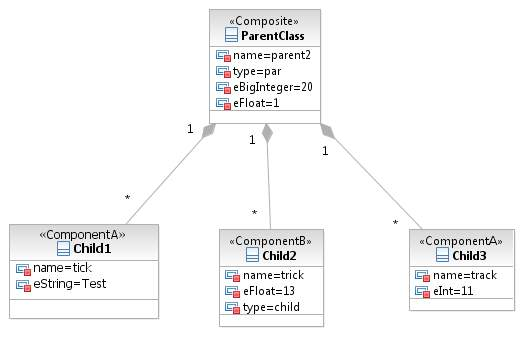
\includegraphics[scale=0.5]{CompareChildrenMatchedOrSimilarTestScreens/Testcase07model2.jpeg}

  \item[testcase\_09:] Es werden 2 voellig unterschiedliche Modelle verglichen.
    
   \begin{equation*}
   Similarity = \frac{0.1+0.2+0.1}{3}=\frac{2}{15}
   \end{equation*}
    
	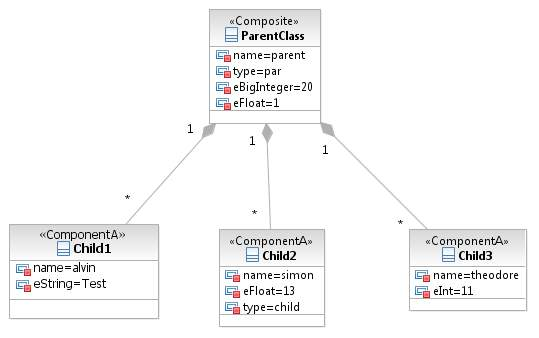
\includegraphics[scale=0.5]{CompareChildrenMatchedOrSimilarTestScreens/Testcase09model1.jpeg}
	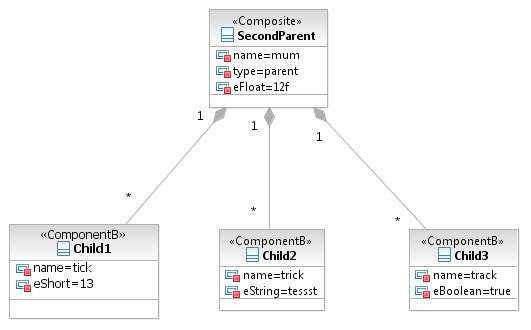
\includegraphics[scale=0.5]{CompareChildrenMatchedOrSimilarTestScreens/Testcase09model2.jpeg}

  \item[testcase\_10:] Es werden 2 voellig unterschiedliche Modelle verglichen. Alle Similarities sind 0.
    
   \begin{equation*}
   Similarity = \frac{0+0+0}{3}=0
   \end{equation*}
    
	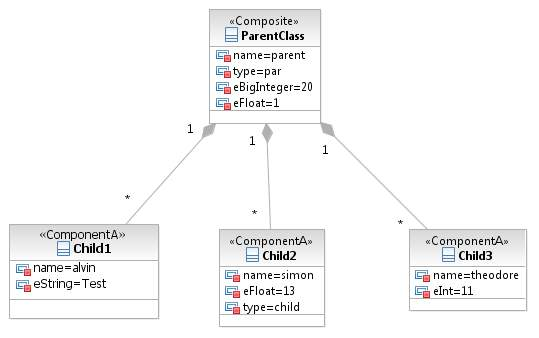
\includegraphics[scale=0.5]{CompareChildrenMatchedOrSimilarTestScreens/Testcase09model1.jpeg}
	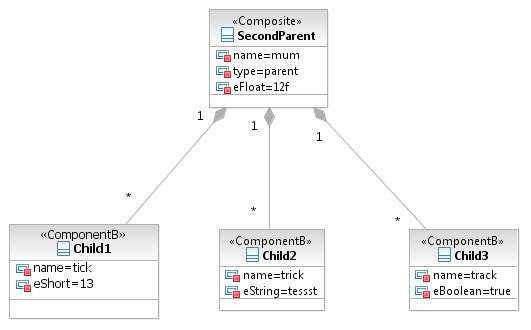
\includegraphics[scale=0.5]{CompareChildrenMatchedOrSimilarTestScreens/Testcase09model2.jpeg}
	\end{description}
	
	



\end{document}